\chapter{ABC}

This chapter will outline a series of illustrative ABC examples. These will serve to demonstrate core concepts touched on in the introduction, demonstrate ABC can sample from complex distributions, and develop the boutique code base which form the foundations of this project. The code for the examples in this section can be found at \url{https://github.com/tomconnell/dram}.\\

\section{Toy problem 1: 1D Gaussian}
As a simple first example consider we have observed $n = 100$ realizations from the Gaussian model $\bm{g_s}(\bm{\theta}) = \frac{1}{\sqrt{2\pi\sigma^2}}\ \text{exp}\Big[\frac{-\mu^2}{2\sigma^2}\Big]$. Our unknown model parameters are $\bm{\theta} = [\mu,\sigma]$. Given we have access to simulation from this model it is possible to leverage ABC algorithms to estimate these unknown model parameters. A synthetic dataset for this problem is created with $\mu = 5$ and $\sigma = 2$. The summary statistics sample mean, $\bar{\mu}$, and sample standard deviation, $\bar{\sigma}$, are used. These provide sufficient statistics with a 1:1 correspondance to the unknown parameters. Figure \ref{toy1-fig1} plots the ABC posterior obtained from using algorithm \ref{ABCrejectionsampler}, the traditional form of an ABC rejection sampler, compared to the analytical likelihood. The metric over summary statistics is evaluated marginally and hence takes the form $\rho = |S_1(\bm{y^*}) - S_1(\bm{y})| +| S_2(\bm{y^*}) - S_2(\bm{y})|$. A uniform prior is used to give equal probability to a bounded area, $p(\mu) = \mathcal{U}(0,10)$ and $p(\sigma) = \mathcal{U}(0,10)$. 
Figure \ref{toy1-fig2} explores the impact of varying the tolerance for this problem.\\

\begin{figure}[H]
	\centering
	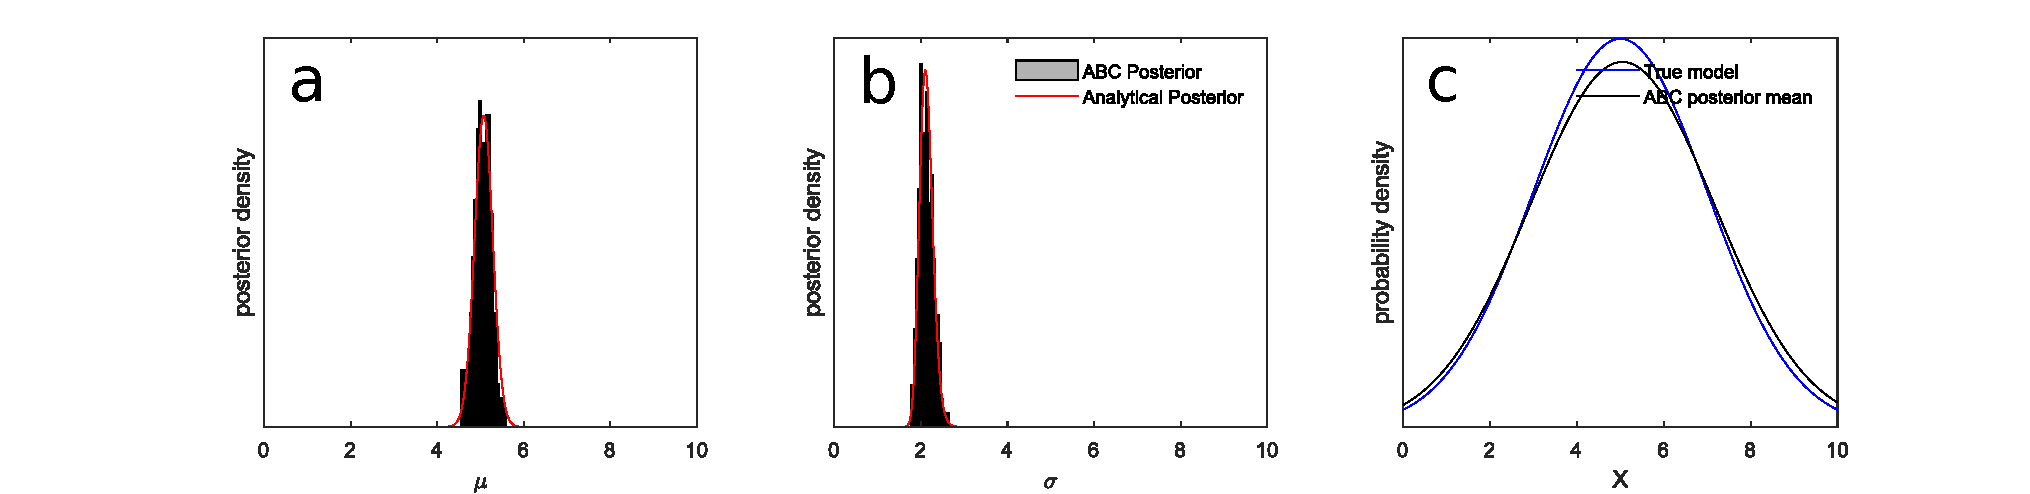
\includegraphics[scale=0.45]{toy1-fig1.pdf}
	\caption{Posterior comparison between ABC and traditional likelihood inference for estimating the parameters, $\bm{\theta} = [\mu,\sigma]$, to a Gaussian model given $n = 100$ observations, $\bm{y}$. The ABC algorithm, algorithm \ref{ABCrejectionsampler}, uses 1 million repititions and a tolerance $\epsilon = 0.1$. The likelihood takes the form $\mathcal{L}(\bm{\theta}|\bm{Y}) = (2\pi\sigma^2)^{-n/2}\ \text{exp}\big[-\frac{1}{2\sigma^2}\sum_{i = 1}^{n}(y_i-\mu)^2\big]$. (a) Marginal posterior compared to marginal ABC posterior for unknown parameter $\mu$. (b) same as (a) but for unknown parameter $\sigma$. (c) Mean ABC posterior model compared to true model.}
	\label{toy1-fig1}
\end{figure}

\begin{figure}[H]
	\centering
	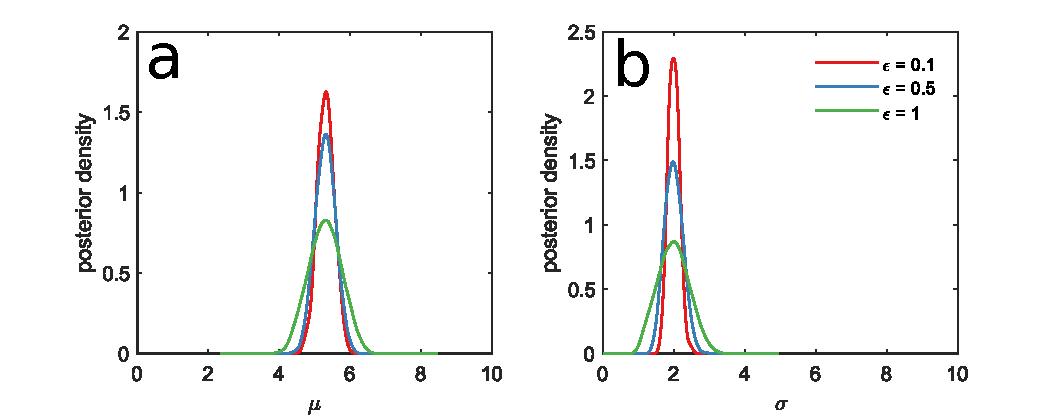
\includegraphics[scale=0.6]{toy1-fig2.pdf}
	\caption{The effect of varying the tolerance $\epsilon$ when estimating $\bm{\theta} = [\mu,\sigma]$ to a Gaussian model given given $n = 100$ observations, $\bm{y}$. Three tolerances are considered, $\epsilon = 0.1$, $\epsilon = 1$, $\epsilon = 5$. (a) Marginal ABC posterior for unknown parameter $\mu$. The true value is $\mu = 5$ (b) same as (a) but for unknown parameter $\sigma$. The true value is $\sigma = 2$}.
	\label{toy1-fig2}
\end{figure}

Figure \ref{toy1-fig1} demonstrates that with sufficient statistics and a low tolerance ABC can accurately resolve the posterior using only the ability to simulate data. However, as figure \ref{toy1-fig2} demonstrates, high tolerances significantly erode posterior accuracy and uncertainty is significantly over-estimated. However, it is true that increasing the tolerance increases the acceptance rate and hence relaxes computational resources. In this case the acceptance rate with $\epsilon = 0.1$ was $0.021\%$, while the acceptance rate with $\epsilon = 1$ was $2.023\%$. Under a model which is expensive to simulate from walking the tightrope between accuracy and efficiency becomes important and needs to be carefully examined. In spite of shortcomings, the strengths of the ABC rejection sampler has led to significant scientific experiments \citep{Fu1997,Weiss1998a,Pritchard1999a}.

\section{Toy problem 2: Linear regression}
\label{sec-lin-reg}

As a second example consider we have observed some data, $\bm{y}$, from the linear model $\bm{g}(\bm{\theta}) = m\bm{x} + b$ and there is some stochasticity in the measurement process such that $\bm{g_s}(\bm{\theta}) = \bm{g}(\bm{\theta}) + \mathcal{N}(0,\sigma^2)$. Our unknown parameters are $\bm{\theta} = [m,b]$, while $\sigma$ is known. In this case it is deemed that computational resources are limitied and MCMC, which uses local transitions, will be needed to improve acceptance rates. MCMC will also be needed when the search spaces are high dimensional, many unknown parameters, and the posterior is a long way from the prior. For this case we can call upon ABC-MCMC in the form of algorithm \ref{ABC-MCMC}. \\

Algorithm \ref{ABC-MCMC} samples the ABC posterior, equation \ref{summary-stat-abc-posterior}. The algorithm relies on evaluating the M-H acceptance probability, equation \ref{M-H-acce}. In our implementations Gaussian transition kernels, $q(.,.)$, are strictly used. As such the transition kernels cancel out in equation \ref{M-H-acce}. That leaves the prior and the weighting kernel to be evalutated at each time step in the Markov chain. The weighting kernel takes the form of equation \ref{generic-weighting-kernel}. In this case a uniform weighting kernel, $K_U$, is implemented. The interpretation of $K_U$ is the same as the accept/reject step in the rejection sampler: 
\begin{equation}
	K_U = 
	\begin{cases}
		1 & \text{if}\ 	\frac{|(S_i(\bm{y^*}) - S_i(\bm{y}))|}				{\epsilon_i} \leq 1\\
		0 & \text{if}\ \frac{|(S_i(\bm{y^*}) - S_i(\bm{y}))|}				{\epsilon_i} > 1
	\end{cases}
\end{equation}
$K_U$ hence forms an indicator function $\mathbbm{1}$ which is equal to $1$ when the distance between statistics, which are fit marginally, is less than the tolerance. Given, $\bm{S} = \{S_1,\dots,S_O\}$, the weighting kernel takes the form:
\begin{equation}
	p(\bm{S}(\bm{y})|\bm{S}(\bm{y^*}),\bm{\theta}) = \prod_{i = 1}^{O} K_U\Big(\frac{\rho(S_i(\bm{y}),S_i(\bm{y^*})}{\epsilon_i}\Big)
	\label{weight-kernel}
\end{equation}
\noindent
As with the 1D Gaussian example it would be possible to take summaries which have a 1:1 correspondance to the unknown parameters. For a given simulation, a linear model could be fit to the simulated data and the slope and intercept used as summaries. However, to demonstrate that this is not necessary, we take inspiration from \citet{vrugt2013toward} and use mean, $\mu$, and standard deviation, $\sigma$, as summary statistics. The slope is restricted to a positive value to make these statistics sufficient. \\

Figure \ref{linear-regression} shows ABC-MCMC applied to the linear regression problem. \\

This example truly highlights how ABC shifts away from many traditional Bayesian and frequentist techniques which rely computing data residuals in the form $\sum (\bm{g}(\bm{\theta})-\bm{y})^2$. This residual is computed in the analytical linear regression likelihood and is at the heart of all likelihood functions which are applied in geophysics, equation \ref{likelihood-1} and equation \ref{likelihood-2}. Instead, ABC opts for informal measures of 'goodness-of-fit' and rely on user-varied tolerances, which guarentee posteriors close-to the true posterior, save for a small degree of bias. The result of a tolerance $> 0$ and summary statistics which do not always measure fitness as tightly as a data residual. However the gain is in diagnostic power. The data residual takes all the information in the data set and mixes it into a single number, the residual value. However, the form of ABC allows for the state of the algorithm at any one stage to be evaluated and fitting statistics marginally means different rules can be set for different statistics depending on what they mean to the inversion. Understanding how statistics change through an inversion, the nature in which they diverge, and the degree to which they spread around the observed value has taught researches in other disciplines a great deal about the nature of their models and the systems in which they study. That same central idea should be transferrable to geophysical parameter estimation problems and may offer room for more diagnostic inversion schemes, one with a greater deal of user control and greated deal of interprebable meaning. \\

In the next section we continue to introduce algorithmic considerations into ABC as we build toward a geophysically relevant parameter estimation system. \\

\begin{figure}[H]
	\centering
	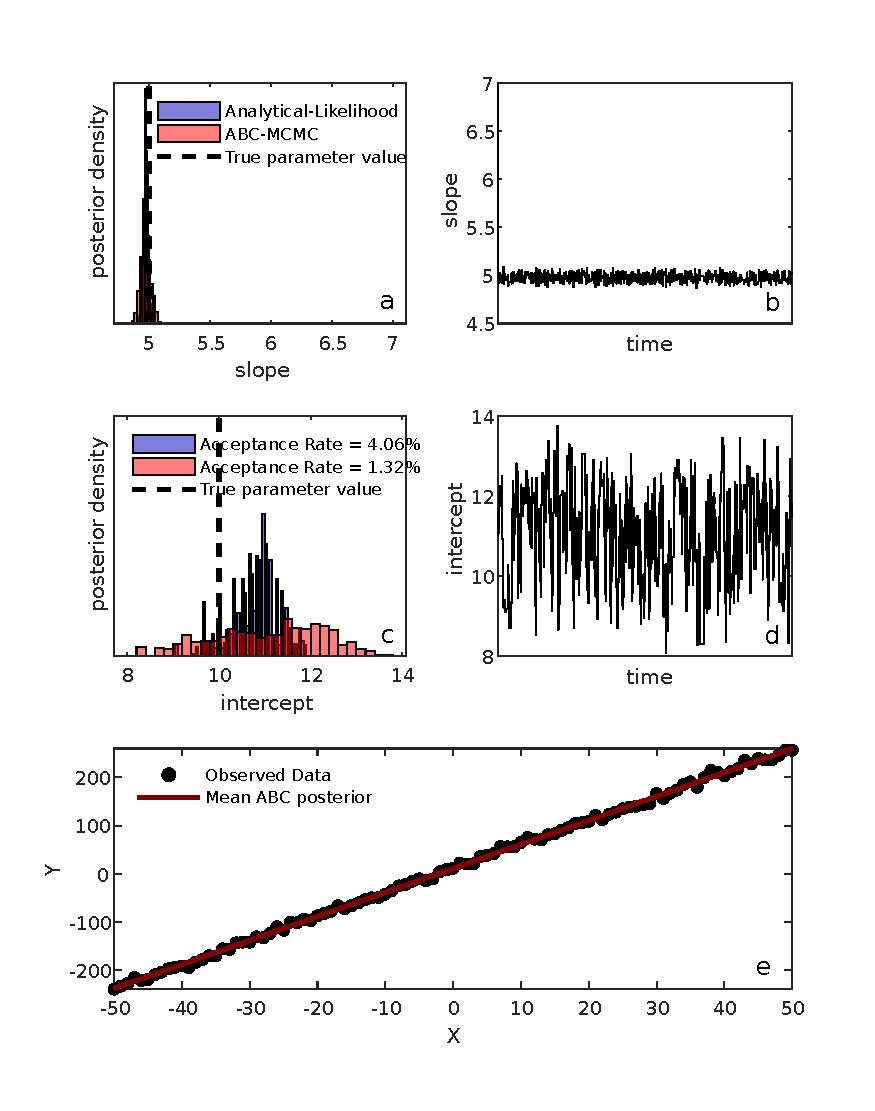
\includegraphics[scale=1.1]{linear-regression-example.pdf}
	\caption{Linear regression with ABC. The ABC posterior is also compared to traditional likelihood machinary. MCMC is used for both posteriors. The tolerance is $\bm{\epsilon} = [2,2]$ and the transition kernel is $q = \mathcal{N}([0,0],I)$. The Markov chain length is $20\ 000$. (a) The marginal ABC posterior and marginal analytical posterior compared for unknown parameter $m$. (b) Plot of Markov chain through time for $m$. (c) Same as (a) except for unknown parameter $b$. (d) Same as (b) except for unknown parameter $b$. (e) Comparison of the mean ABC posterior model and the observed data generated with $m = 5$, $b = 10$ and $\sigma = 5$.}
	\label{linear-regression}
\end{figure}

\section{Toy problem 3: Bivariate Gaussian}
% Introduce the problem
As a third example consider we $n = 100$ observations from a bivariate Gaussian distribution $\mathcal{N}(\bm{\mu},\bm{\Sigma})$ with $\bm{\mu} = \begin{bmatrix}
\mu_X\ \mu_Y
\end{bmatrix}^T$ and $\bm{\Sigma} = \begin{bmatrix}
\sigma^2_X & \rho\sigma_X\sigma_Y\\
\rho\sigma_X\sigma_Y & \sigma^2_Y
\end{bmatrix} $ where both $\bm{\mu}$ and $\bm{\sigma}$ are unknown, hence $\bm{\theta} = [\bm{\mu},\bm{\Sigma}]$. Figure \ref{init-qualms}(a) shows the observed data and the underlying causitive distribution. This example has 5 unknown parameters in total and as such we can appeal to ABC-MCMC for efficient sampling. The weighting kernel takes the same for as equation \ref{weight-kernel} and summaries with a 1:1 correspondance to the unknown parameters are used, the marginal sample means and standard deviations, as well as sample covariance. The prior distribution, $p(\bm{\theta}) = \mathcal{U}(0,10)$, is used to provide equal probability to a bounded area for all unknowns beside correlation, $\rho$, which bounded as $p(\rho) = \mathcal{U}(-1,1)$. Figure \ref{init-qualms}(b) shows the results of the first 10000 time steps from an ABC-MCMC. It can be seen that the algorithm is stationary for the first 3000 repititions.\\

%% Figure a of the observed data and figure b of the stuck chain
\begin{figure}[H]
	\centering
	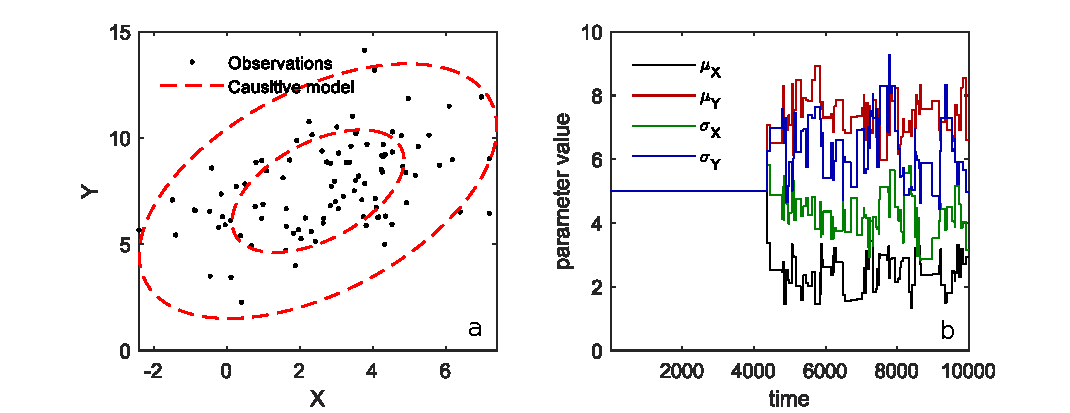
\includegraphics[scale=0.75]{init-problems.pdf}
	\caption{}
	\label{init-qualms}
\end{figure}

%Figure of the chain becoming stuck at the beggining

While ABC-MCMC and the uniform weighting kernel $K_U$ offered invariably improved acceptance rates compared to a rejection scheme in Figure \ref{linear-regression}, it is not without faults. Firstly, it can suffer from an initialisation problem, as highlighted in figure \ref{init-qualms}(b). This is discussed extensively by \citep{Sisson2010a} as they search for solutions which can overcome the initialisation problem, while still using $K_U$. Compounding this, the acceptance rate can rapidly decline past a certain threshold as tolerance is decreased. That is a syptom of the same problem as with initialisation. Each move is either flat out rejected or is determined to be part of the posterior. This makes it prone to becoming stuck when in the tails of a distribution. This is especially problematic in high-dimensional search spaces where the posterior density is an extraordinarily small volume within the parameter space. Ideally, if in a poor spot, the algorithm should be able to make local transitions toward an area of high probability density. However, this adjustment will invove abandoning the uniform kernel. What is needed is a weighting kernel which offers infinite support. That is, the weight dimishes with distance, however it never reaches zero. Fortunately many functions have the required properties. In this text we favour a  weighting kernel based on the Gaussian distribution, $K_G$. The Gaussian distribution is able to be evaluated in a computationally stable way, even as the weighting terms reach extraordinarily small values. See Appendix B for an outline of the stable computational evaluation of the weighting kernel.\\

\begin{figure}
	\centering
	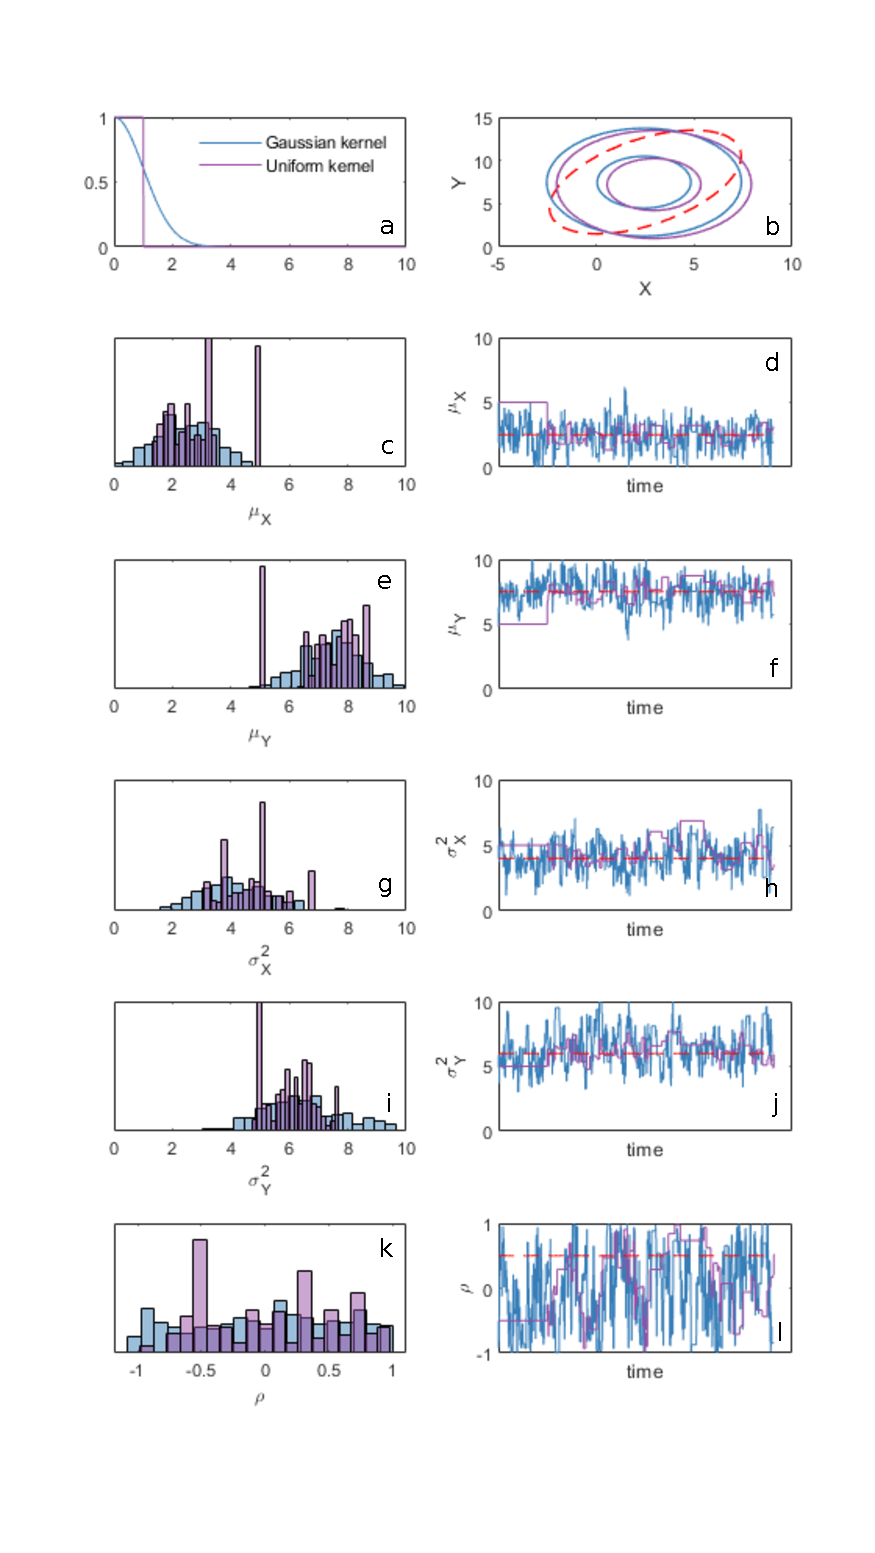
\includegraphics[scale=0.8]{BG7500.pdf}
	\caption{}
\end{figure}

\begin{figure}
	\centering
	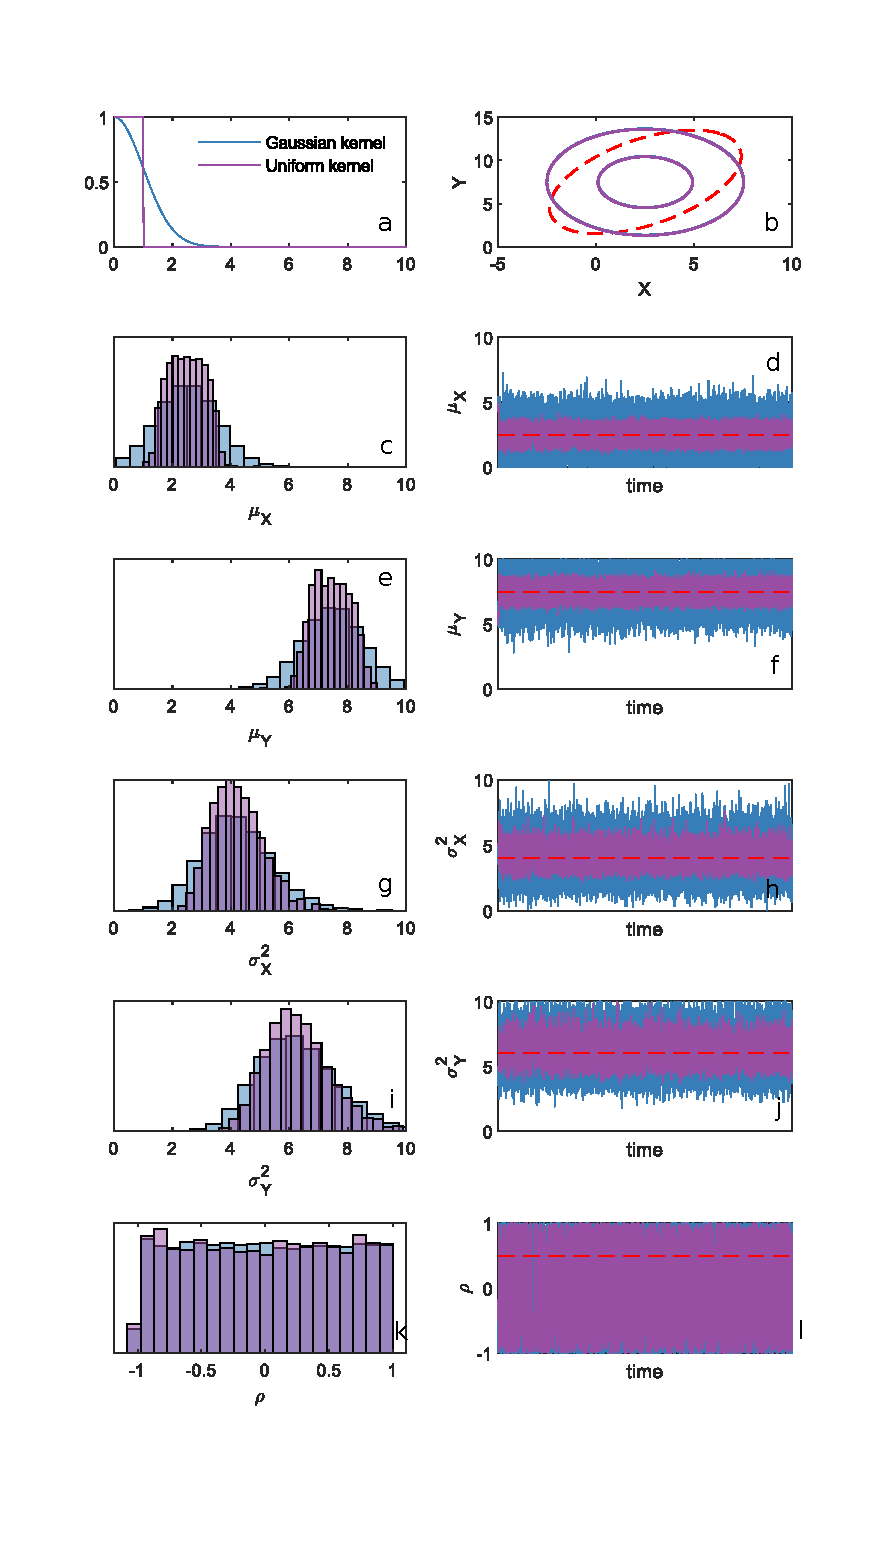
\includegraphics[scale=0.8]{BG1000000.pdf}
	\caption{}
\end{figure}



\section{Toy problem 4: Banana distribution}

%\begin{figure}[H]
%	\centering
%	\def\svgwidth{0.65\columnwidth}
%	\input{image.pdf_tex}
%\end{figure}

 \begin{figure}[H]
 	\centering
	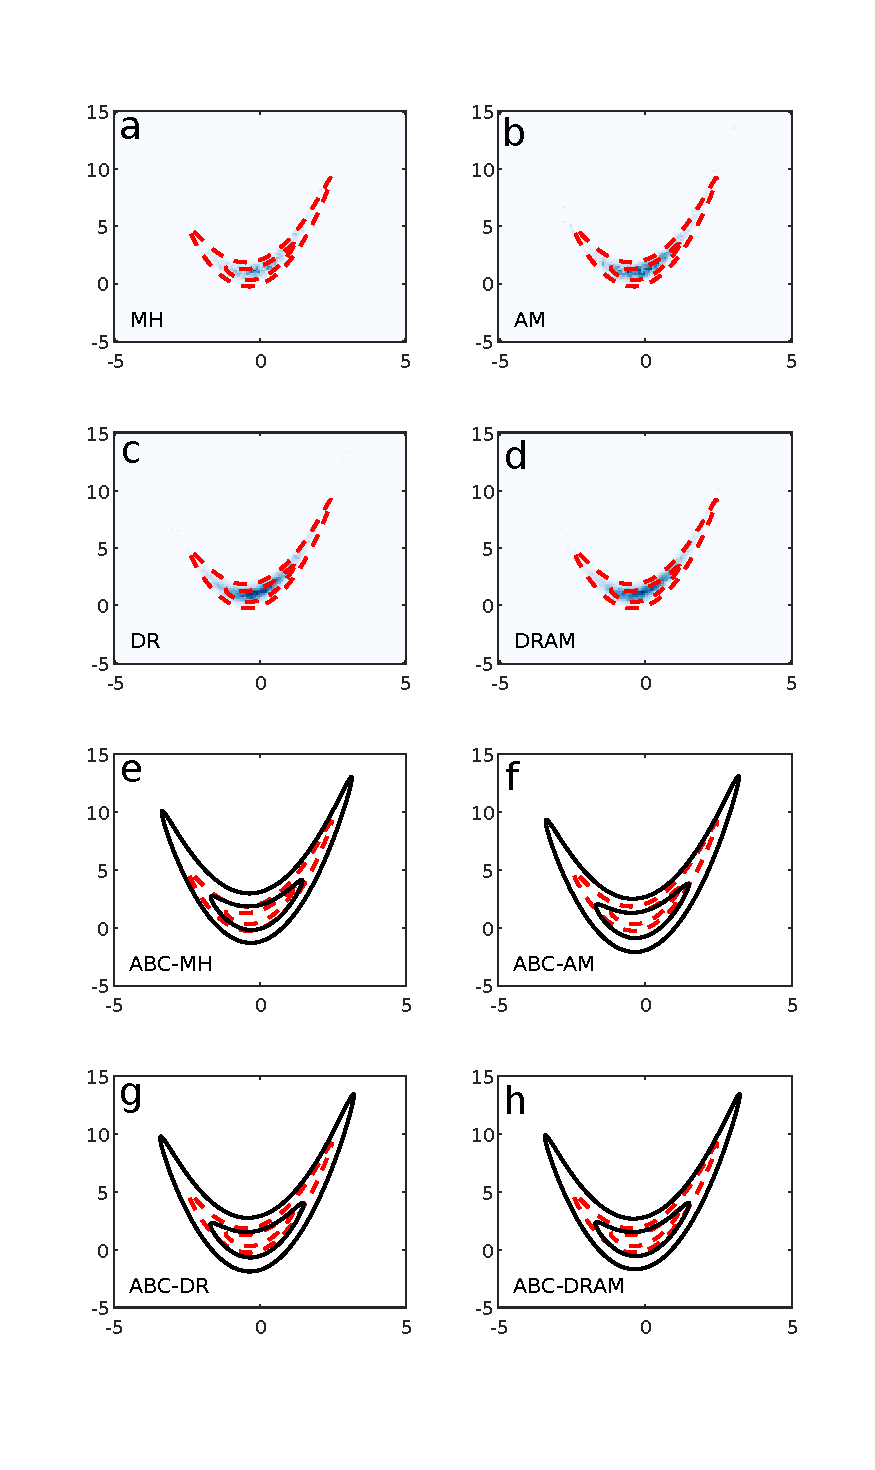
\includegraphics[scale=0.75]{BananaABCvsMCMC.pdf}
 	\caption{Pdf test}
 \end{figure}